\documentclass[11pt]{article}
\usepackage[papersize={2.75in,4.23in},top=.25in,left=.25in, right=.25in, bottom=.25in]{geometry}

%\usepackage{plex-otf} \renewcommand*\familydefault{\sfdefault}

\usepackage{graphicx}\graphicspath{{img/}} 



\usepackage{titlesec}
    \titlespacing{\section}{0ex}{0ex}{0ex}
    \titleformat{\section}[hang]{\bfseries\large}{}{0ex}{}

\setlength{\parindent}{0ex}
\setlength{\parskip}{1ex} 
\newcommand{\grackle}{GRACkLe}

\begin{document} 

\begin{titlepage} % This is the start of the title page.
    \centering 
    {\Huge \grackle} \vskip2ex

    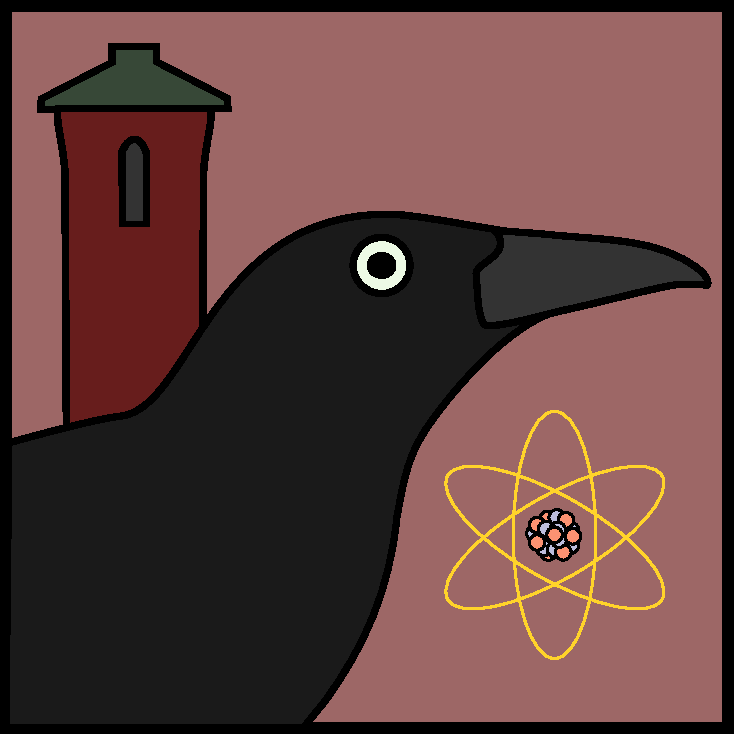
\includegraphics[width=0.75\textwidth]{grackle.pdf}

    \textbf{G}eochemistry \& \textbf{R}adioisotope \textbf{A}nalysis \& \textbf{C}omputation \textbf{L}aboratory

    \rule{2in}{1pt}
    
    We study lakes, ice sheets, environmental change, and the dawn of our solar system.

\end{titlepage} % This is the end of the title page.


\section{Chemistry \& chronology}

A clich\'e in Earth science compares our planet's layers of rocks and sediments to the pages of a book that records Earth's history.
If these layers are the pages, then chemistry is the ink upon them. 

\begin{center}
    \begin{tabular}{cc}
        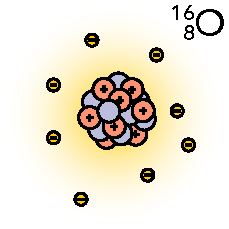
\includegraphics[width=0.4\linewidth]{oxygen-16.pdf}
        &
        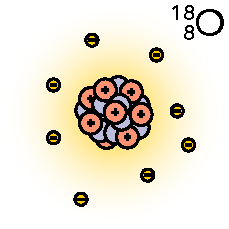
\includegraphics[width=0.4\linewidth]{oxygen-18.pdf}
    \end{tabular}
\end{center}

We measure the elemental and isotopic compositions of rocks and minerals to calculate time and reconstruct process in Earth and planetary systems.

\clearpage
\section{Computation \& statistics}
When reconstructing natural histories from geo- and cosmochemical data, we often rely on mathematical models to relate this data to natural processes. 

We borrow techniques from statistics and computer science to compare models and data and find our best possible guesses of what \emph{actually} happened in nature.

\vfill
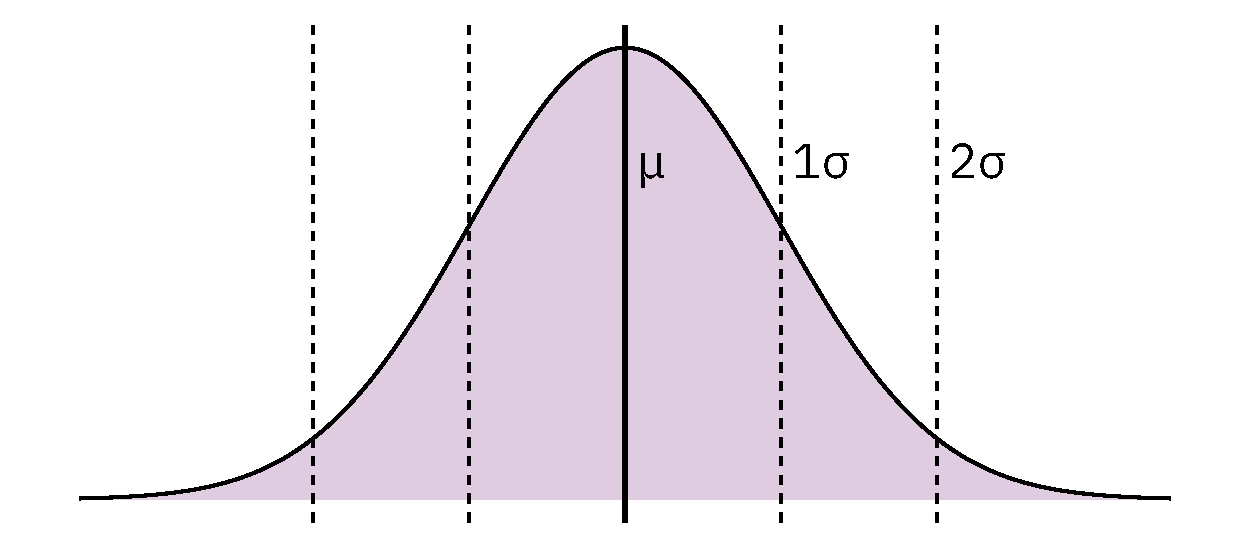
\includegraphics[width=\linewidth]{normal.pdf}
\centerline{\footnotesize The normal distribution of statistics.}

\clearpage
\section{Past environmental change}
We study the deposits of ancient lakes to reconstruct how climate has changed in the past and how environments respond to a changing climate.
We also reconstruct the lifecycles of glaciers, with special emphasis on ice sheet collapse.


\begin{center}\footnotesize
    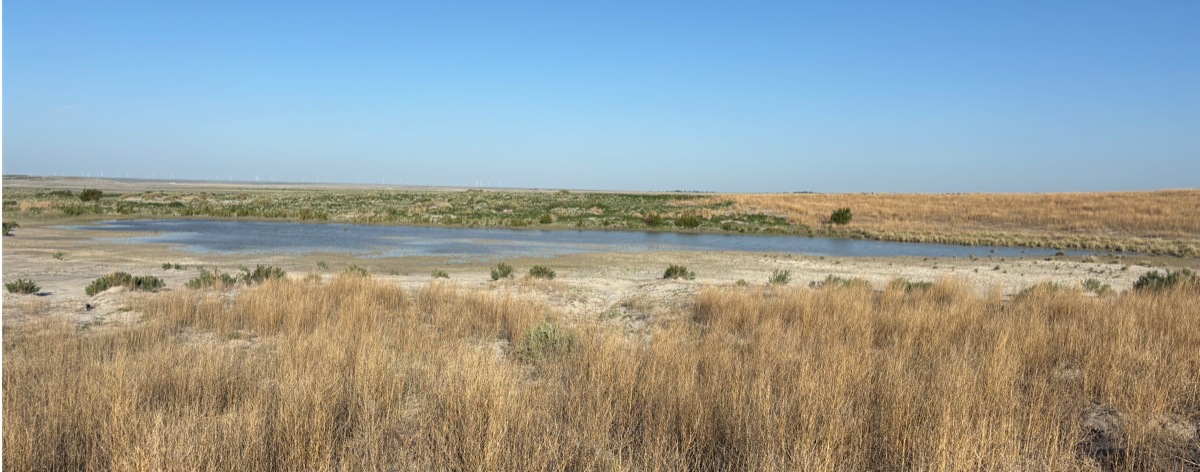
\includegraphics[width=0.9\linewidth]{grulla-water.png}\\ Grulla NWR, New Mexico
    
    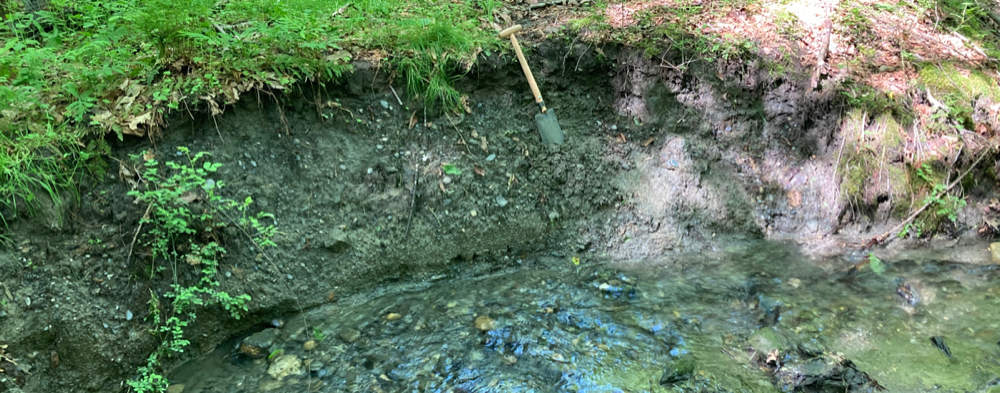
\includegraphics[width=0.9\linewidth]{millbrook.png}\\ Mill Brook, Vermont
\end{center}



\clearpage
\section{Cosmochemistry}
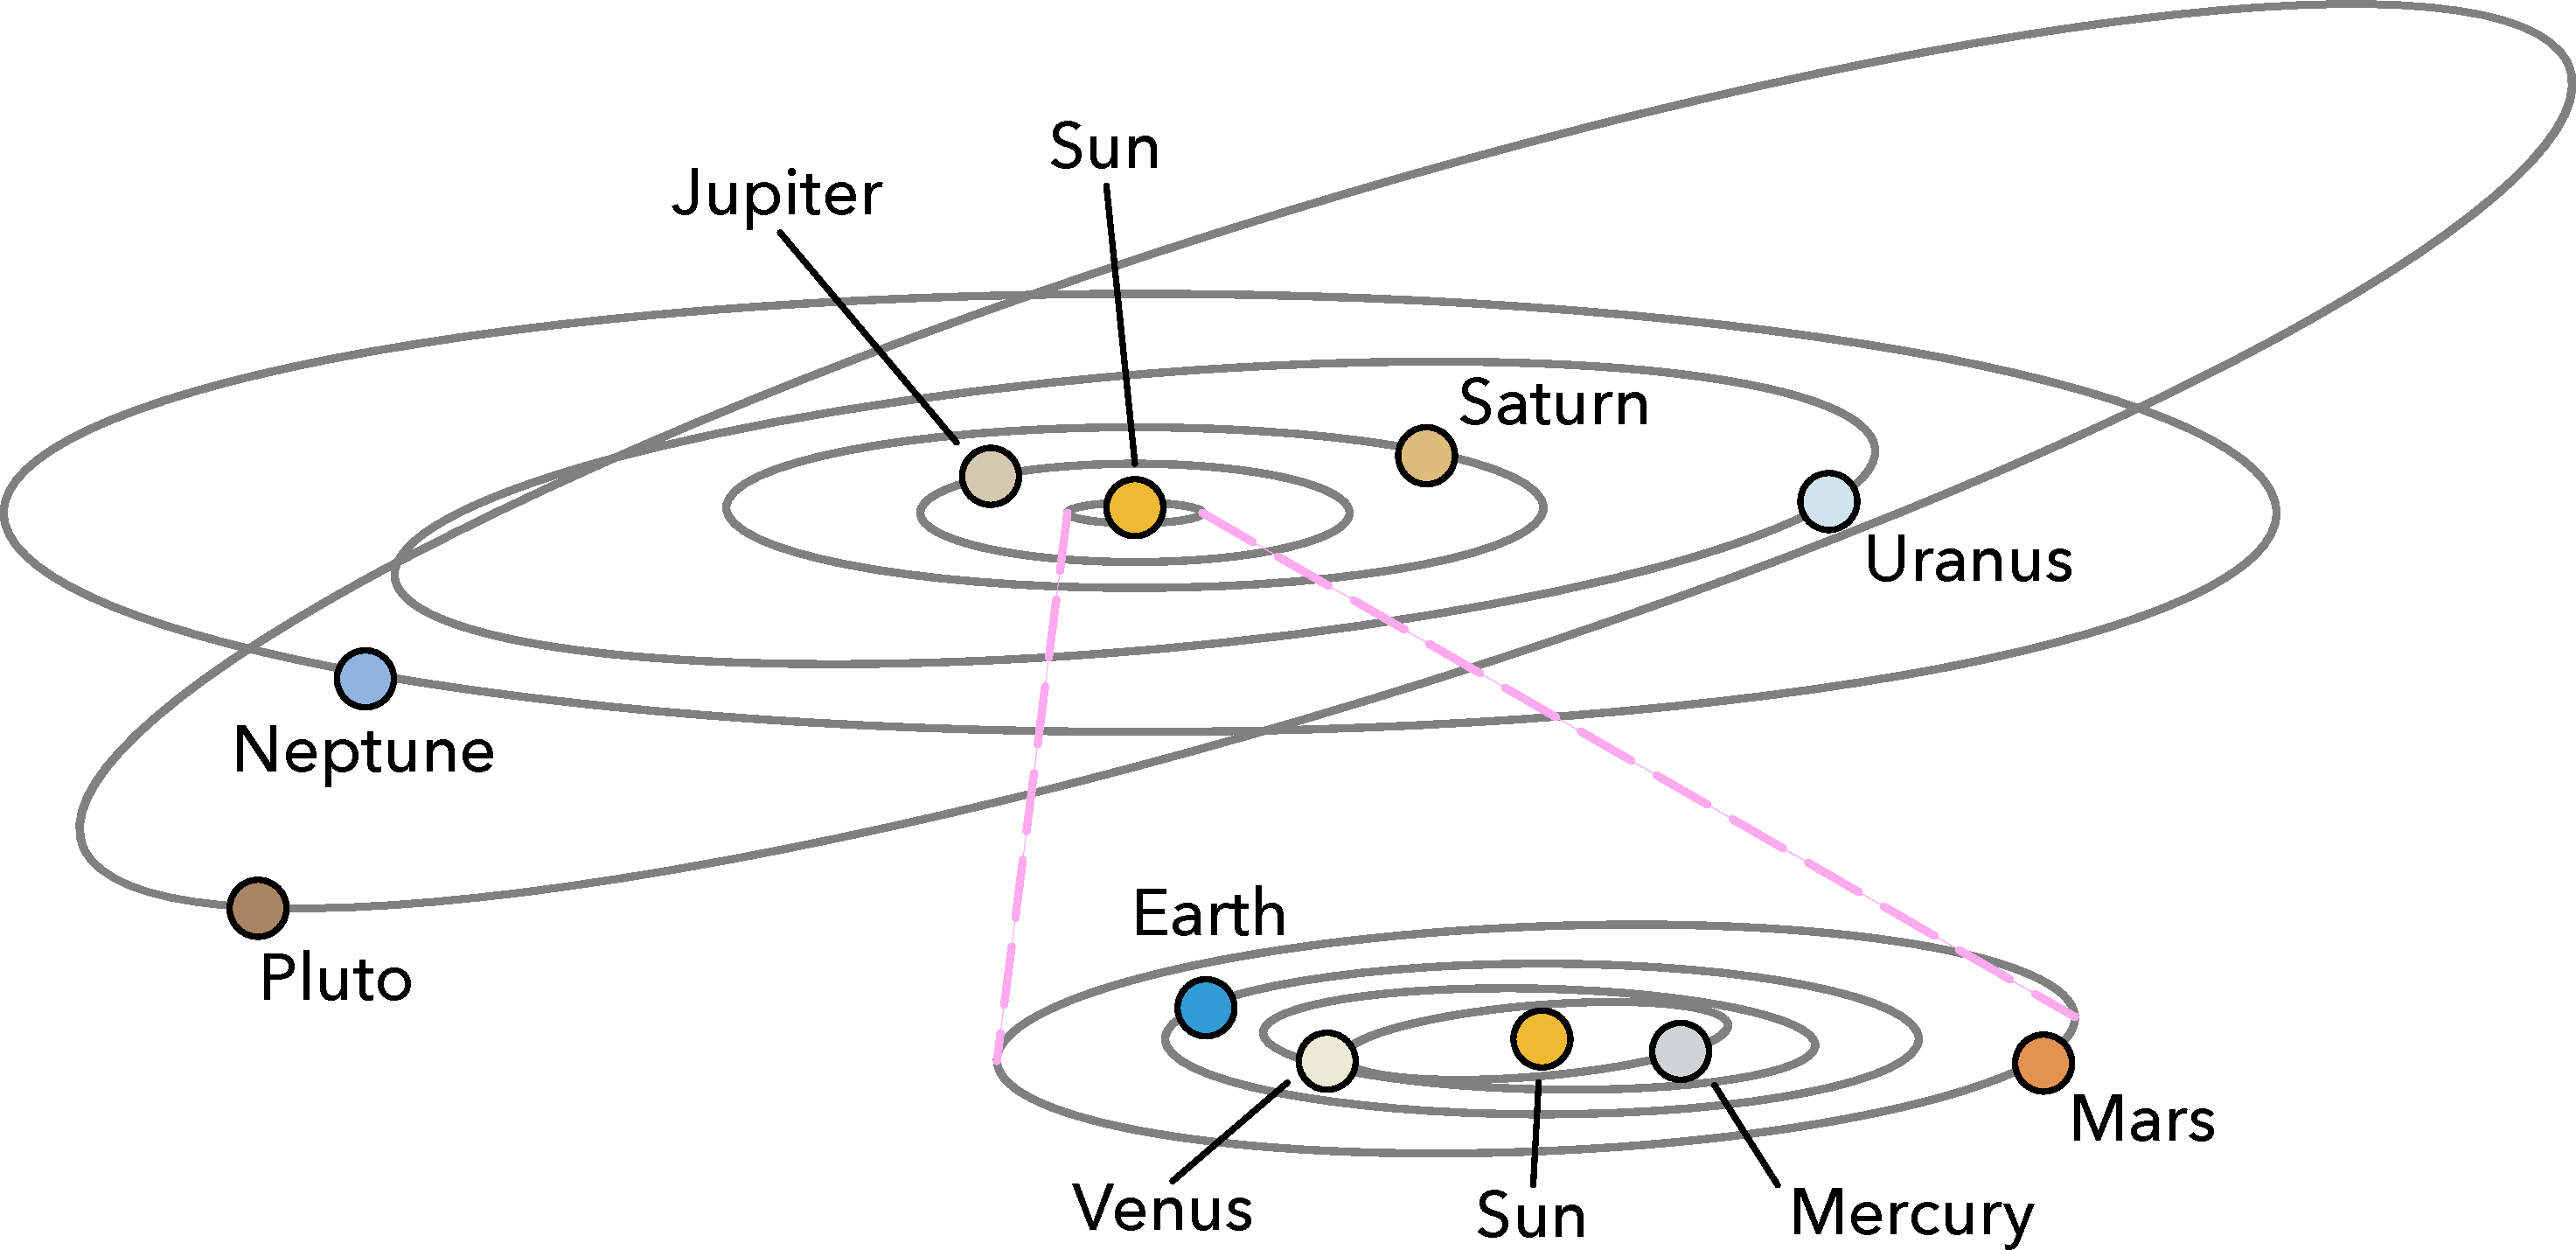
\includegraphics[width=\linewidth]{orbits.pdf}
\vfill
Our solar system\footnote{The solar system includes the Sun and everything that orbits it.} first began to form approximately 4.458 billion years ago from a diffuse cloud of gas and dust. 
We study the chemistry, chronology, and structure of meteorites to reconstruct the formation of our solar system and the first building blocks of the planets. 



\clearpage
\section{Outreach \& museums}

We value scientific communication as much as  scientific knowledge. 

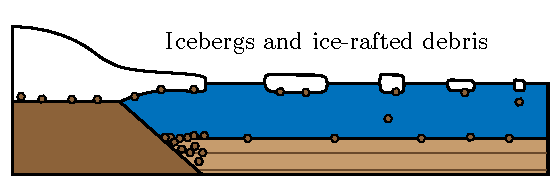
\includegraphics[width=\linewidth]{IRD_diagram.pdf}

\grackle{} scientists involve themselves in public outreach and education.
We have special expertise in exhibit design, collection-based education, and museum outreach. 

\vfill

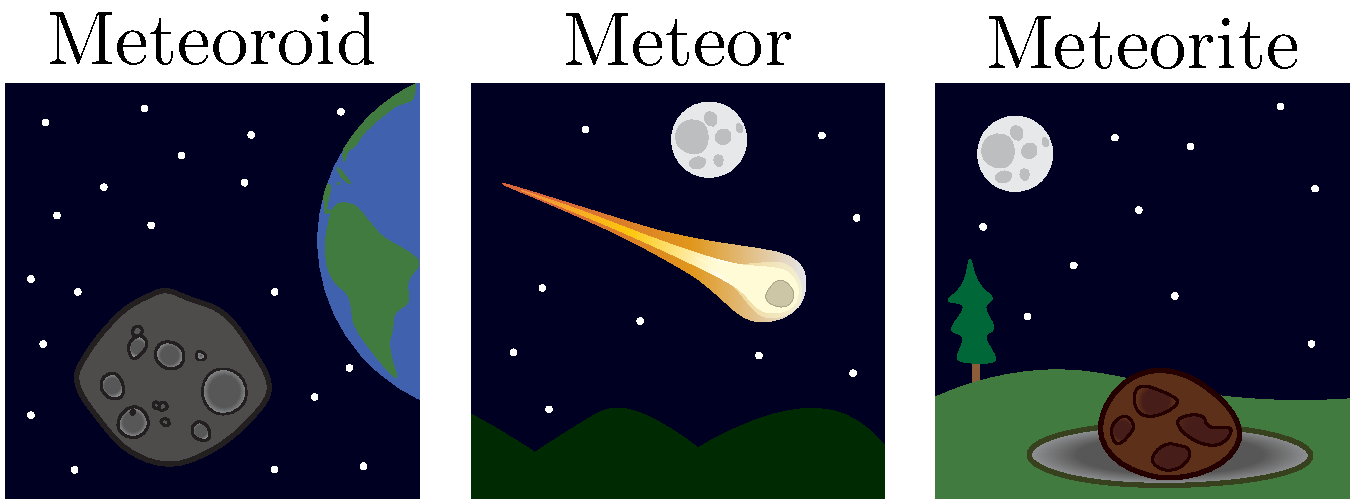
\includegraphics[width=\linewidth]{meteorite.pdf}
\centerline{\footnotesize The many names for rocks from space.}

\clearpage
\section{Graham H.\ Edwards}

I am the \emph{primary investigator} of \grackle, which means that the research and outreach topics in this zine are also my own interests! 
I am fascinated by the timescales, tempo, and evolution of Earth's frozen and flooded environments and our celestial neighborhood.
\begin{center}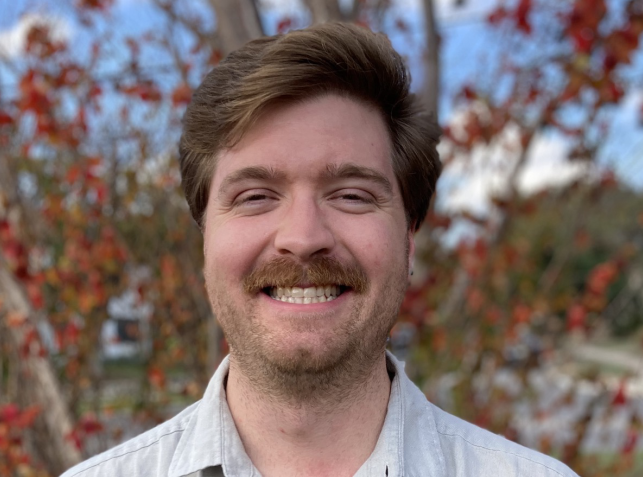
\includegraphics[width=0.6\textwidth]{ghe.png}\end{center}
I am an avid bike commuter and a middling sourdough baker. I adore grackles and vultures.

\clearpage
\section{Want to learn more?}
If you would like to learn more about the research topics and techniques of \grackle{}, first check out the lab website: 

\texttt{https://grackletu.github.io}

\vskip2ex

Please get in touch with me if you would like to discuss a research idea, current \grackle{} research or outreach activities.

\textbf{Email:} \texttt{gedward1@trinity.edu}

\textbf{Office:} Marrs McLean 234

\vfill
\centering
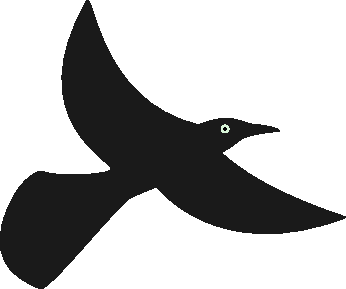
\includegraphics[width=0.4\linewidth]{grackel-silhouette.pdf}

\end{document}

